\section{Cross Section}
\label{sec:AN_CrossSection}

The cross section is computed as described in the beginning of Ch.~\ref{sec:AN_WgMeas}. For comparison purposes, in addition to the measured cross section, we also estimate the cross section based on the signal MC sample which is referred as the MC-based cross section.


The cross section of the whole simulated sample was computed with MCFM in NLO and is for the dedicated signal MC sample $\sigma_1=553.92$~pb. The MC sample was generated with MadGraph, and the cross section in our selected phase space was computed as 

\begin{center}
$\sigma_2 = \sigma_1 \cdot N_2 / N_1$, 
\end{center} 

\noindent{where  $N_2$ and $N_1$ are numbers of events falling into selected phase space and generated in the whole MC sample respectively. For the differential cross section, $N_2$ is number of events falling into specific $P_T^{\gamma}$ bin and to compute }

\begin{center}
\frac{d\sigma }{ dP_T^{\gamma}}, 
\end{center} 

\noindent{we divide over the bin width.} 

Tables~\ref{tab:sc_mc_vs_meas_MUON_WGamma}-\ref{tab:sc_mc_vs_meas_ELECTRON_WGamma} and Fig.~\ref{fig:CS_Wg} summarize the results. The measured cross section agrees with the MC-based cross section within the estimated errors. The measurement is systematically-dominated. 

For additional validation of the measurement procedure, we estimate the cross section of $Z\gamma$ and compare the result with the published CMS result for $Z\gamma$ at~$8$~TeV. The summary of this $Z\gamma$ check is available in App.~\ref{sec:ZgCheck}.

\begin{table}[h]
  \scriptsize
  \begin{center}
  \caption{Cross section and errors. $W\gamma$, muon channel.}
  \begin{tabular}{|c|c|c|}
    bin & $d\sigma/dP_{T}$ &$d\sigma/dP_{T}$ \\ 
    lims & MC based &    meas.       \\ \hline
    total & 9139 & $10949 \pm 91 \pm 2959$ \\ \hline
%    10-15 & 1545 & $1765 \pm 33 \pm 278$ \\ \hline
    15-20 & 754 & $747 \pm 17 \pm 260$ \\ \hline
    20-25 & 382 & $419 \pm 10 \pm 142$ \\ \hline
    25-30 & 210 & $290 \pm 6 \pm 87$ \\ \hline
    30-35 & 129 & $175 \pm 5 \pm 78$ \\ \hline
    35-45 & 70 & $121 \pm 2 \pm 22$ \\ \hline
    45-55 & 36 & $34 \pm 1 \pm 23$ \\ \hline
    55-65 & 23 & $31 \pm 1 \pm 7$ \\ \hline
    65-75 & 13 & $16 \pm 1 \pm 7$ \\ \hline
    75-85 & 9 & $16 \pm 1 \pm 3$ \\ \hline
    85-95 & 6.3 & $9.8 \pm 0.5 \pm 2.4$ \\ \hline
    95-120 & 3.7 & $5.9 \pm 0.3 \pm 1.0$ \\ \hline
    120-500 & 0.27 & $0.41 \pm 0.01 \pm 0.10$ \\ \hline
  \end{tabular}
  \label{tab:sc_mc_vs_meas_MUON_WGamma}
  \end{center}
\end{table}

\begin{table}[h]
  \scriptsize
  \begin{center}
  \caption{Cross section and errors. $W\gamma$, electron channel.}
  \begin{tabular}{|c|c|c|}
    bin & $d\sigma/dP_{T}$ &$d\sigma/dP_{T}$ \\ 
    lims & MC based &    meas.       \\ \hline
    total & 9064 & $9146 \pm 185 \pm 3981$ \\ \hline
%    10-15 & 1550 & $889 \pm 40 \pm 691$ \\ \hline
    15-20 & 749 & $440 \pm 35 \pm 396$ \\ \hline
    20-25 & 375 & $338 \pm 23 \pm 163$ \\ \hline
    25-30 & 210 & $298 \pm 16 \pm 107$ \\ \hline
    30-35 & 129 & $193 \pm 9 \pm 82$ \\ \hline
    35-45 & 71 & $103 \pm 3 \pm 29$ \\ \hline
    45-55 & 34 & $34 \pm 3 \pm 24$ \\ \hline
    55-65 & 22 & $31 \pm 2 \pm 18$ \\ \hline
    65-75 & 14 & $19 \pm 1 \pm 12$ \\ \hline
    75-85 & 9 & $12 \pm 1 \pm 8$ \\ \hline
    85-95 & 6.4 & $10.0 \pm 0.9 \pm 4.3$ \\ \hline
    95-120 & 3.6 & $4.9 \pm 0.4 \pm 2.5$ \\ \hline
    120-500 & 0.26 & $0.46 \pm 0.02 \pm 0.22$ \\ \hline
  \end{tabular}
  \label{tab:sc_mc_vs_meas_ELECTRON_WGamma}
  \end{center}
\end{table}
 
\begin{figure}[htb]
  \begin{center}
   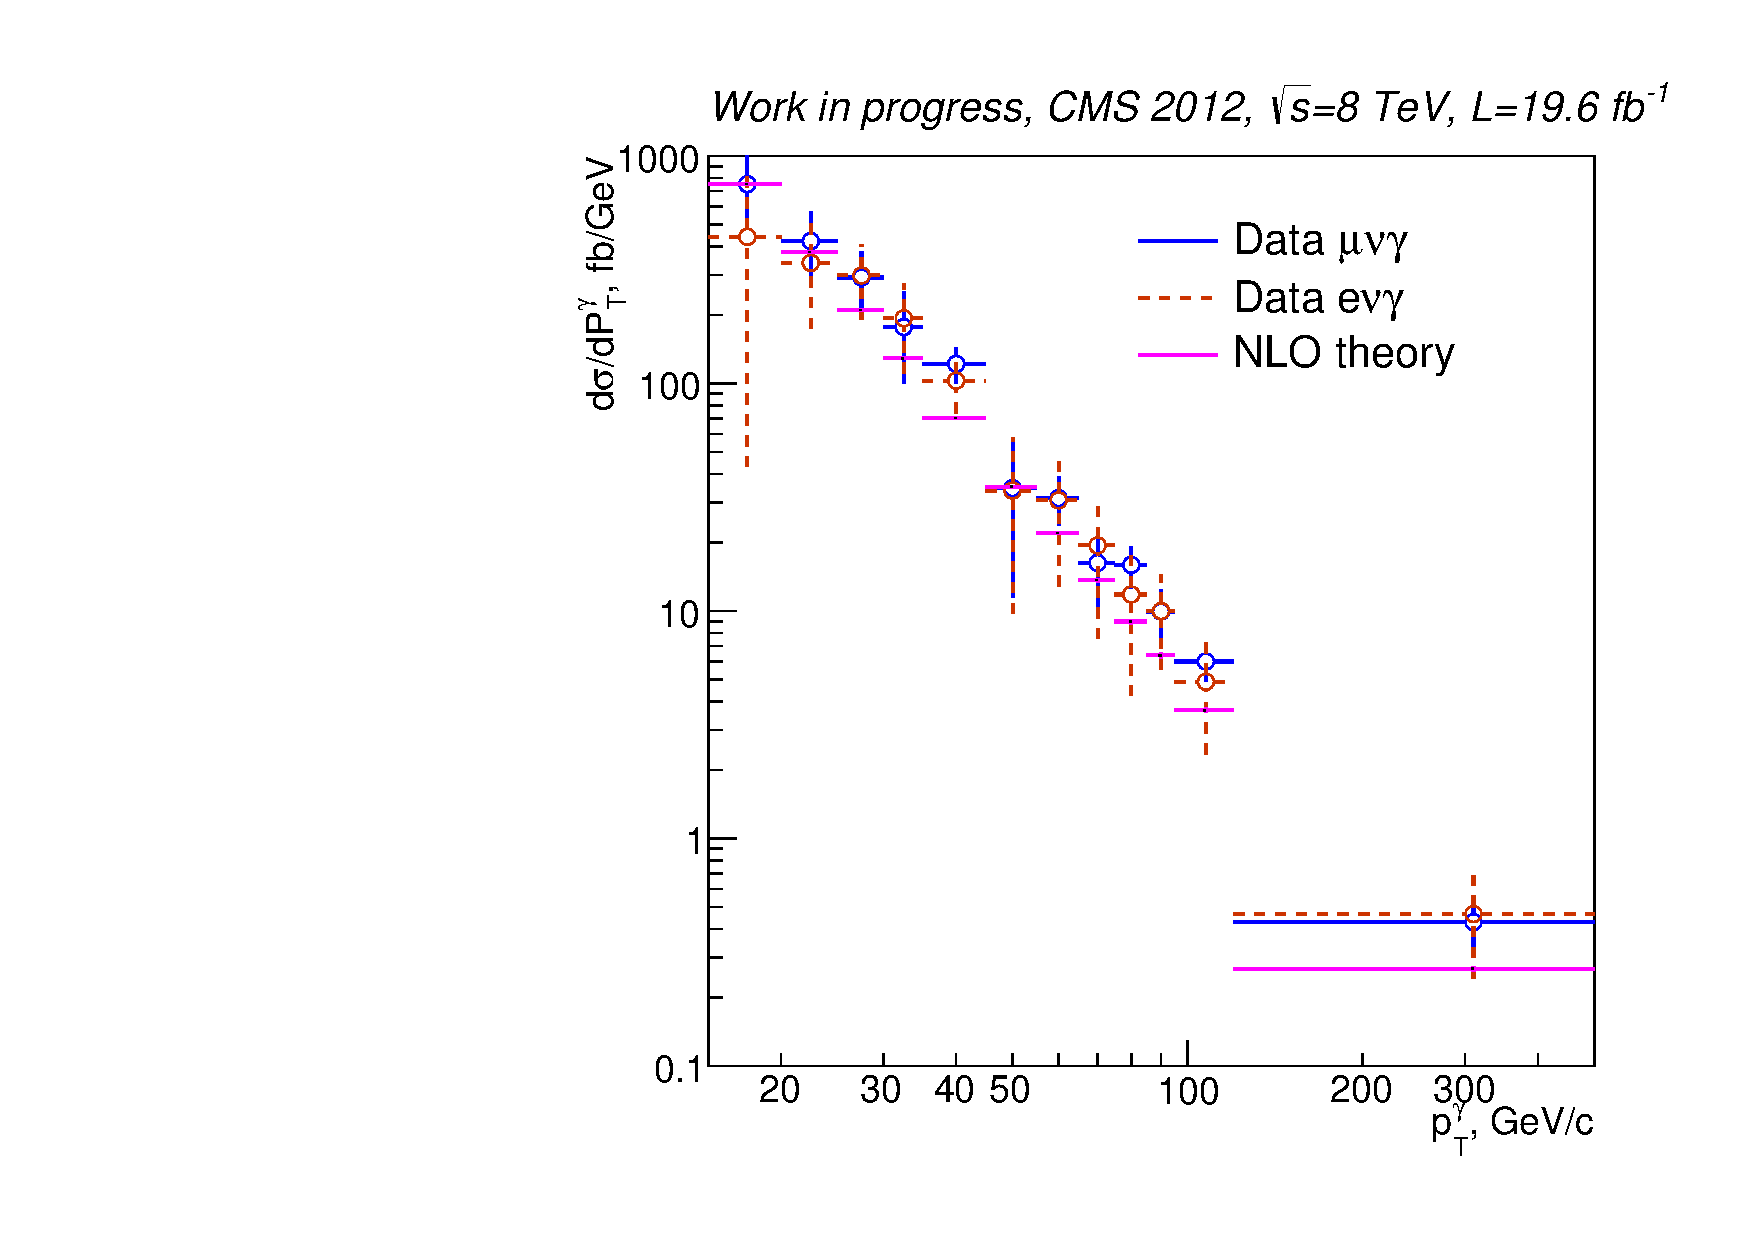
\includegraphics[width=0.5\textwidth]{../figs/figs_v11/ChannelsMERGED_WGamma/CrossSection/compareCSWGamma.pdf}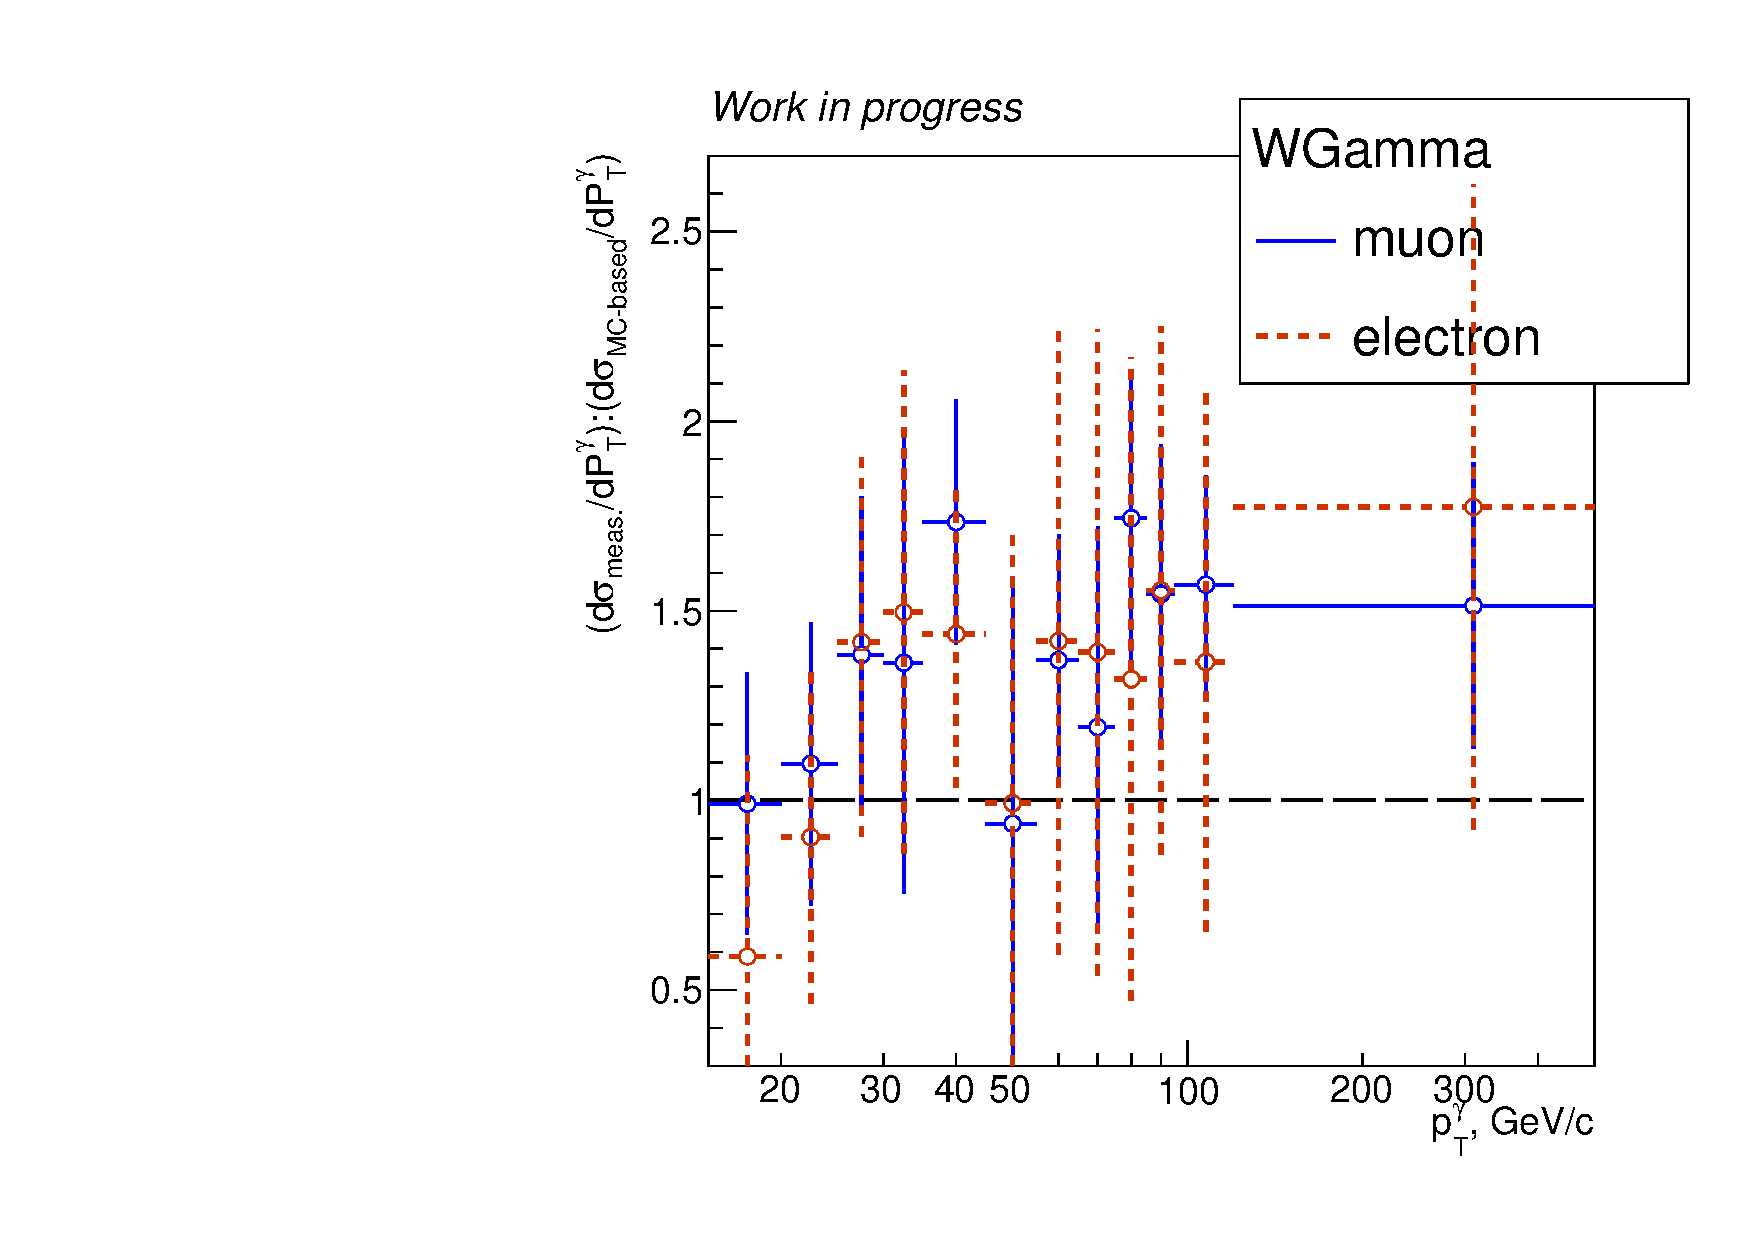
\includegraphics[width=0.5\textwidth]{../figs/figs_v11/ChannelsMERGED_WGamma/CrossSection/compareCSratioTheoryWGamma.pdf}
      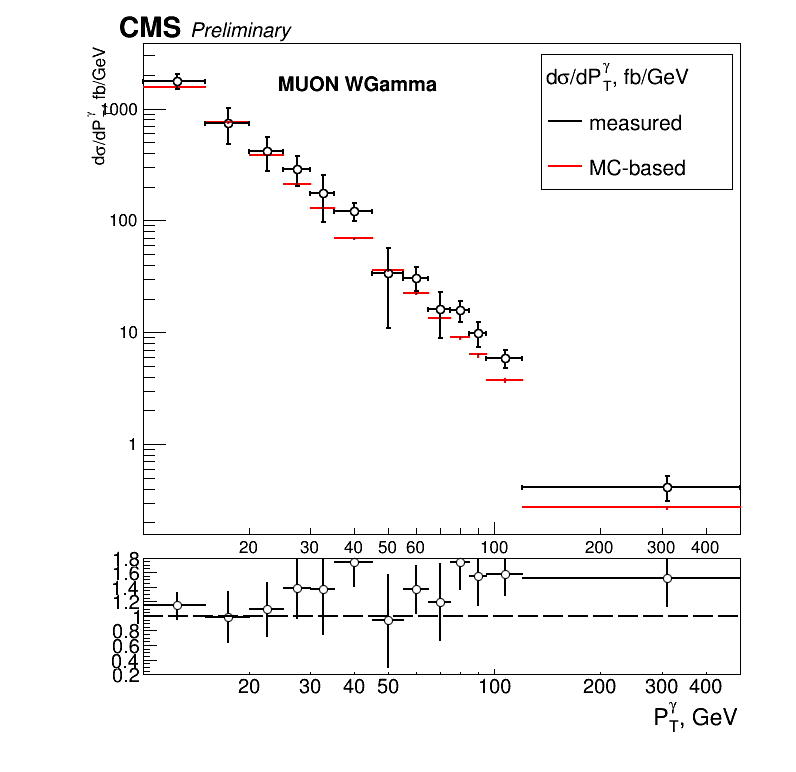
\includegraphics[width=0.48\textwidth]{../figs/figs_v11/MUON_WGamma/CrossSection/c_CS_MUON_WGamma_UNblind.png} 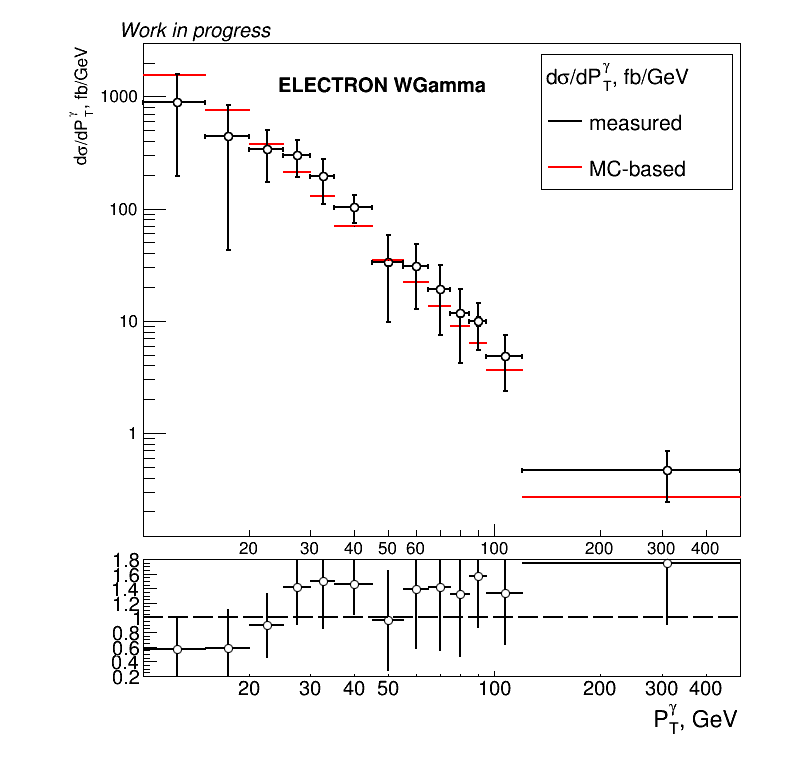
\includegraphics[width=0.48\textwidth]{../figs/figs_v11/ELECTRON_WGamma/CrossSection/c_CS_ELECTRON_WGamma_UNblind.png}
  \caption{$W\gamma$ differential cross section. }
  \label{fig:CS_Wg}
 \end{center}
\end{figure}



